%----------------------------------------------------------------------------------------
%	PACKAGES AND OTHER DOCUMENT CONFIGURATIONS
%----------------------------------------------------------------------------------------

\documentclass[12pt]{article}

%%%%%%%%%%%%%%%%%%%%%%%%%%%%%%%%%%%%%%%%%
% Lachaise Assignment
% Structure Specification File
% Version 1.0 (26/6/2018)
%
% This template originates from:
% http://www.LaTeXTemplates.com
%
% Authors:
% Marion Lachaise & François Févotte
% Vel (vel@LaTeXTemplates.com)
%
% License:
% CC BY-NC-SA 3.0 (http://creativecommons.org/licenses/by-nc-sa/3.0/)
% 
%%%%%%%%%%%%%%%%%%%%%%%%%%%%%%%%%%%%%%%%%

%----------------------------------------------------------------------------------------
%	PACKAGES AND OTHER DOCUMENT CONFIGURATIONS
%----------------------------------------------------------------------------------------

\usepackage{amsmath,amsfonts,stmaryrd,amssymb} % Math packages

\usepackage{enumerate} % Custom item numbers for enumerations

\usepackage[ruled]{algorithm2e} % Algorithms

\usepackage[framemethod=tikz]{mdframed} % Allows defining custom boxed/framed environments

\usepackage{listings} % File listings, with syntax highlighting
\lstset{
	basicstyle=\ttfamily, % Typeset listings in monospace font
}

%----------------------------------------------------------------------------------------
%	DOCUMENT MARGINS
%----------------------------------------------------------------------------------------

\usepackage{geometry} % Required for adjusting page dimensions and margins

\geometry{
	paper=a4paper, % Paper size, change to letterpaper for US letter size
	top=2.5cm, % Top margin
	bottom=3cm, % Bottom margin
	left=2.5cm, % Left margin
	right=2.5cm, % Right margin
	headheight=14pt, % Header height
	footskip=1.5cm, % Space from the bottom margin to the baseline of the footer
	headsep=1.2cm, % Space from the top margin to the baseline of the header
	%showframe, % Uncomment to show how the type block is set on the page
}


%----------------------------------------------------------------------------------------
%	COMMAND LINE ENVIRONMENT
%----------------------------------------------------------------------------------------

% Usage:
% \begin{commandline}
%	\begin{verbatim}
%		$ ls
%		
%		Applications	Desktop	...
%	\end{verbatim}
% \end{commandline}

\mdfdefinestyle{commandline}{
	leftmargin=10pt,
	rightmargin=10pt,
	innerleftmargin=15pt,
	middlelinecolor=black!50!white,
	middlelinewidth=2pt,
	frametitlerule=false,
	backgroundcolor=black!5!white,
	frametitle={Command Line},
	frametitlefont={\normalfont\sffamily\color{white}\hspace{-1em}},
	frametitlebackgroundcolor=black!50!white,
	nobreak,
}

% Define a custom environment for command-line snapshots
\newenvironment{commandline}{
	\medskip
	\begin{mdframed}[style=commandline]
}{
	\end{mdframed}
	\medskip
}

%----------------------------------------------------------------------------------------
%	FILE CONTENTS ENVIRONMENT
%----------------------------------------------------------------------------------------

% Usage:
% \begin{file}[optional filename, defaults to "File"]
%	File contents, for example, with a listings environment
% \end{file}

\mdfdefinestyle{file}{
	innertopmargin=1.6\baselineskip,
	innerbottommargin=0.8\baselineskip,
	topline=false, bottomline=false,
	leftline=false, rightline=false,
	leftmargin=2cm,
	rightmargin=2cm,
	singleextra={%
		\draw[fill=black!10!white](P)++(0,-1.2em)rectangle(P-|O);
		\node[anchor=north west]
		at(P-|O){\ttfamily\mdfilename};
		%
		\def\l{3em}
		\draw(O-|P)++(-\l,0)--++(\l,\l)--(P)--(P-|O)--(O)--cycle;
		\draw(O-|P)++(-\l,0)--++(0,\l)--++(\l,0);
	},
	nobreak,
}

% Define a custom environment for file contents
\newenvironment{file}[1][File]{ % Set the default filename to "File"
	\medskip
	\newcommand{\mdfilename}{#1}
	\begin{mdframed}[style=file]
}{
	\end{mdframed}
	\medskip
}

%----------------------------------------------------------------------------------------
%	NUMBERED QUESTIONS ENVIRONMENT
%----------------------------------------------------------------------------------------

% Usage:
% \begin{question}[optional title]
%	Question contents
% \end{question}

\mdfdefinestyle{question}{
	innertopmargin=1.2\baselineskip,
	innerbottommargin=0.8\baselineskip,
	roundcorner=5pt,
	nobreak,
	singleextra={%
		\draw(P-|O)node[xshift=1em,anchor=west,fill=white,draw,rounded corners=5pt]{%
		Question \theQuestion\questionTitle};
	},
}

\newcounter{Question} % Stores the current question number that gets iterated with each new question

% Define a custom environment for numbered questions
\newenvironment{question}[1][\unskip]{
	\bigskip
	\stepcounter{Question}
	\newcommand{\questionTitle}{~#1}
	\begin{mdframed}[style=question]
}{
	\end{mdframed}
	\medskip
}

%----------------------------------------------------------------------------------------
%	WARNING TEXT ENVIRONMENT
%----------------------------------------------------------------------------------------

% Usage:
% \begin{warn}[optional title, defaults to "Warning:"]
%	Contents
% \end{warn}

\mdfdefinestyle{warning}{
	topline=false, bottomline=false,
	leftline=false, rightline=false,
	nobreak,
	singleextra={%
		\draw(P-|O)++(-0.5em,0)node(tmp1){};
		\draw(P-|O)++(0.5em,0)node(tmp2){};
		\fill[black,rotate around={45:(P-|O)}](tmp1)rectangle(tmp2);
		\node at(P-|O){\color{white}\scriptsize\bf !};
		\draw[very thick](P-|O)++(0,-1em)--(O);%--(O-|P);
	}
}

% Define a custom environment for warning text
\newenvironment{warn}[1][Warning:]{ % Set the default warning to "Warning:"
	\medskip
	\begin{mdframed}[style=warning]
		\noindent{\textbf{#1}}
}{
	\end{mdframed}
}

%----------------------------------------------------------------------------------------
%	INFORMATION ENVIRONMENT
%----------------------------------------------------------------------------------------

% Usage:
% \begin{info}[optional title, defaults to "Info:"]
% 	contents
% 	\end{info}

\mdfdefinestyle{info}{%
	topline=false, bottomline=false,
	leftline=false, rightline=false,
	nobreak,
	singleextra={%
		\fill[black](P-|O)circle[radius=0.4em];
		\node at(P-|O){\color{white}\scriptsize\bf i};
		\draw[very thick](P-|O)++(0,-0.8em)--(O);%--(O-|P);
	}
}

% Define a custom environment for information
\newenvironment{info}[1][Info:]{ % Set the default title to "Info:"
	\medskip
	\begin{mdframed}[style=info]
		\noindent{\textbf{#1}}
}{
	\end{mdframed}
}
 % Include the file specifying the document structure and custom commands

%----------------------------------------------------------------------------------------
%	ASSIGNMENT INFORMATION
%----------------------------------------------------------------------------------------

\title{\textbf{Comparing and Analyzing the Effectiveness of Various String Matching Algorithms Across Different Domains}} % Title of the assignment

\author{\textbf{Research Question -} How do different string \and matching algorithms perform across various application domains, \and and what factors contribute to their varying effectiveness?} % Author name and email address

\date{\textbf{Words}: not enough} % University, school and/or department name(s) and a date

%----------------------------------------------------------------------------------------

\begin{document}

\doublespacing

\maketitle % Print the title
\thispagestyle{empty}
\pagebreak
\tableofcontents
\thispagestyle{empty}

\clearpage
\pagenumbering{arabic}

\pagebreak
\section{Introduction} % Unnumbered section

The impacts and applications of string matching algorithms extend far beyond their immediate textual applications; its quotidian use in domains such as bioinformatics, web crawling and security systems make it a pertinent area of study within computer science. There is also constant research being carried out to identify more efficient algorithms, and find ways in which to combine them with other disciplines to carry out certain tasks.

For instance, multiple studies have been recently published performing various comparative analyses of new string matching algorithms \parencite{4}, and their applicability to a wide range of domains such as biological sequences \parencite{5}, quantum computing \parencite{6}, and instrusion detection systems \parencite{7}. These findings indicate the modern-day relevance and applicability of string matching algorithms and demonstrate its worthiness as a subject of investigation.

Similarly, this paper seeks to adopt an investigative style by examining \textbf{how different string matching algorithms perform across various application domains, and the factors that contribute to their varying effectiveness}. 

To formulate a methodology that will directly address this aim, the research question can be broken down into three parts: measuring the performance of the mentioned string algorithms, analyzing the results by making links back to the theory in order to the understand the reasons behind their varying efficiency, and linking these to different domains.

To examine this subject, three popular string matching algorithms were programmed and tested on their ability to carry out three tasks from three different domains. They are then evaluated on a set of criteria to determine their efficiency and applicability. To maintain focus on the research question, the reasoning and rationale behind all the decisions will be explained to demonstrate how they directly address the question.

The choice of this research question is both relevant and justifiable, reflecting the persistent demand for evaluating and optimizing string matching algorithms across a range of applications.

\section{Theoretical Background} % Numbered section
\subsection{Topic Overview}
\parencite{3} String matching algorithms (often used interchangeably with string or pattern searching
algorithms) are a subset of string algorithms. The term is composed of three parts:
“string”, “matching”, and “algorithm”. Strings refer to an abstract data type consisting
of a sequence of characters. Matching relates to it's function to identify specific patterns
within a larger dataset that match a criteria. As for algorithms, these can be defined as a set of instructions designed to carry out a function. These algorithms take in two
inputs: a pattern ($P$), which is a sequence of characters being searched for within a larger
sequence, a text ($T$). Within string matching problems, there exists two general variants
\parencite{2}:

\begin{enumerate}
	\item \textbf{Find occurences of a pre-defined pattern in a previously unseen dataset} \\
	Carried out using finite automata models \parencite{2} (an idealized machine used to recognize
	patterns in a given text; it accepts or rejects the input depending on whether the
	pre-defined pattern occurs in the text) or through the combinatorial properties of
	strings.
	\item \textbf{Find occurences of any identifiable patterns in a given text} \\
	Carried out using finite automata and binary trees.
\end{enumerate}

Linking into the mentioned problem variants, these algorithms can be further classified into two categories \parencite{1}: exact, and approximate string matching algorithms. As
its name suggests, the former refers to finding occurences of a pattern that match it to
the character, whereas the latter allows for some variation or deviation. For the purpose
of this investigation, the first problem variant, as well as an exact-string matching approach was chosen for all the algorithms, both for simplicity and control. Three exact
string matching algorithms were chosen for comparison based on their popularity: Naive,
Knuth-Morris-Pratt, and Rabin-Karp. Prior to their explanations, it is important to note
that the following notation will be used:

\begin{table}[htbp]\caption{String Matching Algorithm Notation}
\begin{center}% used the environment to augment the vertical space
% between the caption and the table
\begin{tabular}{r c p{10cm} }
\toprule
$m$ & $=$ & Length of $P$\\
$n$ & $=$ & Length of $T$\\
$T_{j}$ & : & For an input text $T$ where $0 \le j \le n - 1$\\
$P_{i}$ & : & For an input pattern $P$ where $0 \le i \le m - 1$\\
\bottomrule
\end{tabular}
\end{center}
\label{tab:StringMatchinAlgorithmNotation}
\end{table}

\subsection{Naive Algorithm}

\parencite{8} Also known as the “brute-force” approach, this algorithm compares the first indexes
of both $P$ and $T$. If $P_{i}$ equals $T_{j}$ then $i$ and $j$ are incremented and further compared. If
$P_{i}$ reaches $m - 1$ then a variable containing the number of occurences of $P$ is incremented
and $P_{i}$ is reset to $P_{i=0}$. On the other hand, if they do not match, then $P_{i}$ is reset and
$j$ incremented. This repeats until $T_{j=m-1}$ is reached. Since there is no pre-processing
phase, the only time complexity taken into account is during its matching phase, which
is expected to be $O(n \cdot m)$ \parencite{2}. The algorithm is better expressed in pseudocode:

\begin{center}
\begin{singlespace}
\begin{minipage}{0.75\linewidth}
\begin{algorithm}[H]
	$n \leftarrow T.length()$ \;
	$m \leftarrow P.length()$ \;

	\bigskip

	\For{$i \leftarrow 0$ \bf{to} $n-m$}{
		\While{$j < m$ \bf{and} $P[j] == T[i+j]$}{
			$j \leftarrow j + 1$}
		\If{$j == m$}{
			\textbf{output} "Pattern found at index" + $i$}
	}
	\caption{Naive}
\end{algorithm}
\end{minipage}
\end{singlespace}
\end{center}

A practical example is also illustrated:

\begin{figure}[H]
	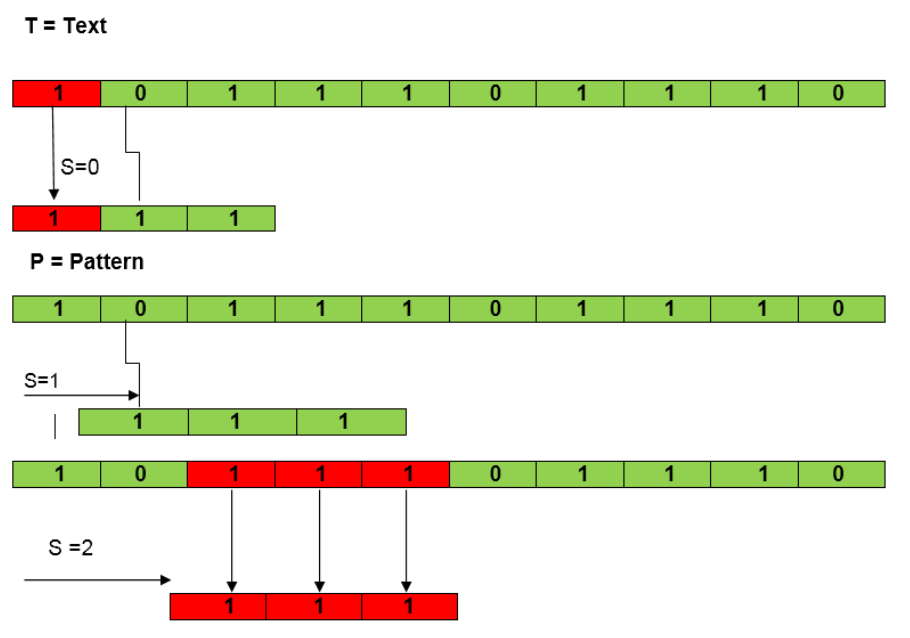
\includegraphics[scale=0.6]{naive_figure}
	\centering
	\caption{Illustrated Naive \parencite{11}}
\end{figure}

As can be seen, both indexes for the pattern (111) and the text (1011101110) begin at 0 and their first characters are compared. As they match, the indexes are incremented for both P and T and their respective characters matched. As they do not, the index for the pattern is reset to 0 and the text's index incremented. In the depicted example, this is repeated twice more before a match is found -- everytime the index of the pattern increases, it matches with the increasing text index.

The best case scenario of this process is when $P_{i=0}$ is not present in $T$, yielding an
$O(n)$ number of comparisons, making it particularly advantageous for solving problems
with small $n$ and $m$ values. When larger sets are used however, the algorithm's efficiency significantly deteriorates. The worst case scenario for instance would be when
all the characters for $P$ and $T$ are the same (${P_{i=0} \ldots P_{m-1}} = {T_{j=0} \ldots T_{n-1}}$) or
when all the characters for both $P$ and $T$ are the same except for their last characters ($({P_{i=0} \ldots P_{m-2}} = {T_{j=0} \ldots T_{n-2}}) \land (P_{m-1} = T_{n-1})$). This would yield an
$O(m \cdot (n - m + 1))$ number of comparisons.


\subsection{Knuth-Morris-Pratt Algorithm}

\parencite{2} \parencite{9} This algorithm differs from the Naive approach by implementing an LPS table
as part of the pre-processing phase. Its purpose is to keep track of the comparisons made;
after a mismatch, it is used to calculate where to begin the next match without needing
to reset $P$. The table is constructed by determining the largest prefix of $P$ that matches
its largest suffix -- the main idea is to identify how many characters can be skipped, by not
matching characters that have already been calculated to match (eliminating redundancy).
Although appearing complicated, this can be better explained through pseudocode and a
practical example represented through a truth table. Upon initalization, the LPS table is
an array of 0s of length $m$. For demonstration purposes, $P$ will equal "$ABABA$":

\begin{table}[!htbp]
    \centering
    \begin{tabular}{|c|c|c|c|}
        \hline
        Index ($i$) & Pattern Character ($P_{i}$) & Length (of Suffix-Prefix match) & LPS Value ($LPS[i]$) \\
        \hline
        0 & A & 0 & 0 \\
        1 & B & 0 & 0 \\
        2 & A & 0 & 1 \\
        3 & B & 1 & 2 \\
        4 & A & 2 & 3 \\
        \hline
    \end{tabular}
    \caption{Truth Table for Pattern "ABABA"}
\end{table}

\begin{center}
\begin{singlespace}
\begin{minipage}{0.75\linewidth}
\begin{algorithm}[H]
	$length \leftarrow 0$ \;
	$LPS \leftarrow m * [0]$ \;

	\bigskip

	\While{$i < m$}{
		\If{$P[i] == P[m]$}{
			$length \leftarrow length + 1$\;
			$LPS[i] \leftarrow 0$\;
			$i \leftarrow i + 1$\;
		}
		\ElseIf{$length \neq 0$}{
			$length \leftarrow LPS[length - 1]$\;
		}
		\Else{
			$LPS[i] \leftarrow 0$\;
			$i \leftarrow i + 1$\;
		}
	}

	\textbf{return} $LPS$
	\caption{CalculateLPSArray}
\end{algorithm}
\end{minipage}
\end{singlespace}
\end{center}

Afterwards, the main phase involves applying the calculated LPS table on $T$. The
indexes $i$ and $j$ both begin at 0, and are incremented while $P_{i}$ matches $T_{j}$. When a
mismatch occurs, it becomes apparent that the characters in $P$ match with the characters
of $T$ up to the mismatch ($P_{0 \ldots (i-1)} = T_{j-i \ldots j-1}$). Moreover, from the LPS table, it is known
that $LPS[i - 1]$ represents the length of the longest part of the prefix and suffix of $P$.
With these pieces of information, it can be concluded that the characters in $P_{0 \ldots i-1}$ do
not need to be checked with $T_{j-i \ldots j-1}$ since it is already known that they match. Thus,
these can be skipped in both $P$ and $T$. The exact process is presented in pseudocode here
below:

\begin{center}
\begin{singlespace}
\begin{minipage}{0.75\linewidth}
\begin{algorithm}[H]
	$n \leftarrow T.length()$ \;
	$m \leftarrow P.length()$ \;
	$LPS \leftarrow CalculateLPSArray(P)$ \;
	$i \leftarrow 0$ \;
	$j \leftarrow 0$ \;

	\bigskip

	\While{$j < n$}{
		\If{$P[i] == T[j]$}{
			$i \leftarrow i + 1$\;
			$j \leftarrow j + 1$\;
		}
		\If{$i == m$}{
			\textbf{output} "Pattern found at index" $+ (j-i)$\;
			$i \leftarrow LPS[i-1]$\;
		}
		\ElseIf{$j < n$ \textbf{and} $P[i] \neq T[j]$}{
			\If{$i \neq 0$}{
				$i \leftarrow LPS[i - 1]$\;}
			\Else{
				$j \leftarrow j + 1$\;
			}
	}}
	\caption{KMP Match}
\end{algorithm}
\end{minipage}
\end{singlespace}
\end{center}

A practical example is also illustrated:

\begin{figure}[H]
	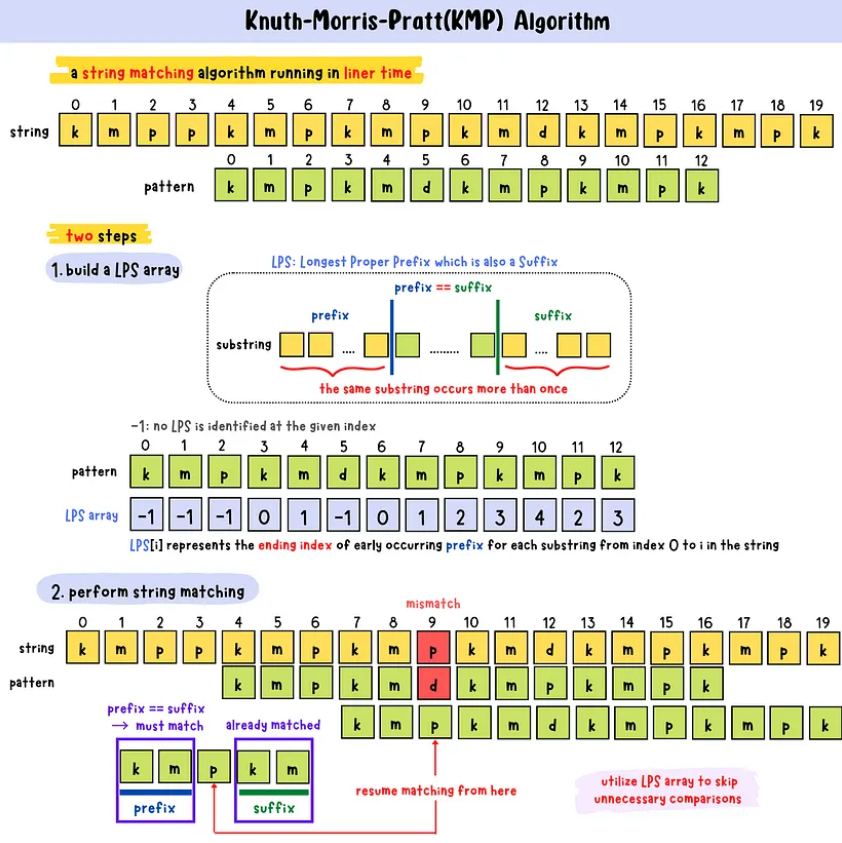
\includegraphics[scale=0.7]{kmp_figure}
	\centering
	\caption{Illustrated KMP \parencite{12}}
\end{figure}

Firstly, the pattern is pre-processed to create an LPS table. This works by iterating through each character of the pattern, and determining its earliest occurrence within it. For example, beginning with “k”, it is its first instance in the pattern and so there is no other earliest occurrence, so it is registered in the LPS table as -1, to indicate that there are not any. This repeats for the next 2 characters. Upon reaching index 3 with “k”, it is noticed that its earliest instance now exists and is found at index 0, and so it is registered in the LPS table as so. This process continues for the rest of the pattern. Afterwards, the “longest proper prefix which is also a suffix” is found by taking the longest sub-list of consecutive LPS values. In this case it would be indexes 6 to 1 (kmpkmp). This array is then used as part of the string matching to skip the unnecessary comparisons (in the example, since it is known that the prefix equals the suffix, when kmpkmd is reached, the next 7 characters can be skipped, since based on the LPS table they are known not to match).

By skipping the unecessary character comparisons, the algorithm proves to be much
more efficient than the Naive approach. This is seen in its worst-case time complexity,
which is $O(n + m)$ (best-case time complexity remains the same). As for the time complexities in the pre-processing and matching phases, they are $O(m)$ and $O(n)$ respectively.

\subsection{Rabin-Karp Algorithm}

\parencite{10} The most similar out of the two to the Naive approach, the Rabin-Karp algorithm
has a similar process of checking every substring for a match. Unlike the Naive approach
however, this algorithm compares “hash values”. These are calculated using rolling hash
functions, which allow for the removal and introduction of characters to the calculation,
eliminating the need to recalculate the value entirely from scratch. To perform the hashing
process on a substring, the following steps are carried out:

\begin{question}[\bf{Rolling Hash Function}]
\begin{enumerate}
	\item The base $(b)$ and modulus $(p)$ values are chosen (usually prime numbers).
	\item A hash value is initialised to 0 and the initial hash value of $P$ calculated (for each character in $P$, its contribution is added to the hash value as $c \cdot (b^{m-i-1}) \% p$).
	\item The hash value for the first substring of length $m$ in $T$ is calculated.
	\item Everytime $j$ is incremented, the contribution of the leftmost character is removed, the contribution of the rightmost character added.
	\item Compare the text and pattern matches each time; if they match then it is a \textbf{potential match} (rolling function outputs can be the same for different inputs). To verify the match, a character match is performed.
	
\end{enumerate}
\end{question}

The time complexity for the pre-processing phase (calculating $P$'s hash value) is $O(m)$.
As for the time complexities in the matching phase, they are $O(m \cdot n)$ for the worst case
scenario and $O(n + m)$ for the expected case. Although this algorithm maintains the
simplicity of the Naive algorithm all the while improving its efficiency, it has a disadvantage that, depending on the specific $T$ case, may impact its efficiency -- a spurious
hit. This refers to the case where a hash value match is made between $P$ and $T$ but the
characters do not match, increasing the time complexity. This can however be minimized
by implementing a robust hash function.

The pseudocode for the algorithm is presented here below:

\begin{center}
\begin{singlespace}
\begin{minipage}{0.75\linewidth}
\begin{algorithm}[H]
	$n \leftarrow T.length()$ \;
	$m \leftarrow P.length()$ \;
	$h \leftarrow 1$ \;
	$hashT \leftarrow 0$ \;
	$hashP \leftarrow 0$ \;

	\bigskip

	\For{$i \leftarrow 1$ \textbf{to} $m-1$}{
		$h \leftarrow (h \cdot b) \% p$ \;
	}

	\bigskip

	\For{$i \leftarrow 0$ \textbf{to} $m-1$}{
		$hashP \leftarrow (b \cdot hashP + P[i]) \% p$ \;
		$hashT \leftarrow (b \cdot hashT + T[i]) \% p$ \;
	}

	\bigskip

	\For{$i \leftarrow 0$ \textbf{to} $n - m$}{
		$match \leftarrow TRUE$ \;

		\For{$j \leftarrow 0$ \textbf{to} $m - 1$}{
			\If{$P[j] \neq T[i + j]$}{
				$match \leftarrow FALSE$ \;
			}
		}

		\If{$match == TRUE$}{}
			\textbf{output} "Pattern found at index " $+ i$\;
		\If{$i < n - m$}{
			$hashT \leftarrow (b \cdot hashT + T[i]) + T[i + m] \% p$ \;
			\If{$hashT < 0$}{
				$hashT \leftarrow hashT + p$ \;
			}
		}
	}
\caption{Rabin Karp}
\end{algorithm}
\end{minipage}
\end{singlespace}
\end{center}

A practical example is also illustrated:

\begin{figure}
    \centering
    \subfloat[\centering Pattern Hash Code]{{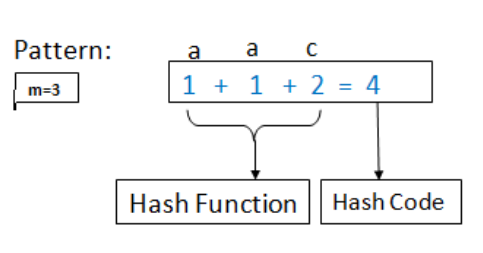
\includegraphics[scale=0.55]{rabin_karp_figure1} }}
    \qquad
    \subfloat[\centering Comparison With Text]{{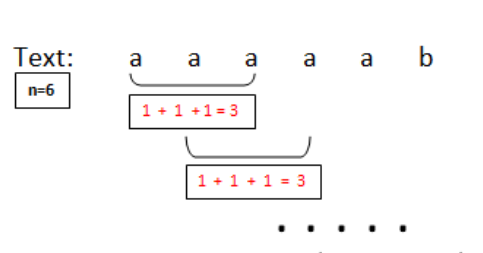
\includegraphics[scale=0.55]{rabin_karp_figure2} }}
    \caption{Illustrated Rabin Karp \parencite{13}}
\end{figure}

To aid with comprehension, the rolling hash function used to calculate hash values is replaced with a simplified hashing function: each character is converted to its numerical position within the alphabet (e.g. a = 1, b = 2). Since it is known that the pattern length is $m$ = 3, the hash values of groups of 3 characters are calculated from the text each time. Using the predefined assigned hash values for the characters, the pattern's hashcode is calculated to yield 4. This means that for each sub-group within the text that is examined, its hashcode should yield 4 to be deemed a potential match. In the example, the hashcode for the first group examined (aaa) is calculated (3). Since they do not match, the second sub-group is checked (aaa). This continues up until the end of the text, where no match is found.

\section{Experimental Methodology}

\subsection{Measuring Performance}

To measure the detailed algorithms' performance, their mentioned pseudocode algorithms were programmed in $Python$ $3.12$. 
Python was chosen due to it's wide array of third-party modules, three of which are used as part of the implementation: $time$, $matplotlib$ and $cProfile$. 
$time$ is used to measure the algorithms' runtimes for each algorithm, $matplotlib$ is used to generate the graphical plots, and $cProfile$ is used to calculate the time and space-complexities of the programs.
An experimental methodology was chosen as their is limited secondary data available due to the high specificity of the task. Furthermore, this methodology provides increased control over variable manipulation.
Using their implementations, the following variables will be measured:

\begin{enumerate}
	\item \textbf{Dependent Variables} \\
	\underline{Pre-processing runtime (ms)} - The amount of time taken to prepare the data prior to matching.\\
	\underline{Matching runtime (ms)} - The amount of time taken to search a pattern $P$ in a text $T$.\\
	\underline{Total number of comparisons} - The total number of references made to the text (until all instances of the pattern are found) \\
	\underline{Total number of comparisons with unmatching characters} - The total number of references made to the text for characters that do not match (until all instances of the pattern are found).
	\item \textbf{Control Variables} \\
	\underline{Language} - Depending on whether the language employs a compiler or an interpetor, runtime speeds can differ. Moreover, the type of programming language (procedural, functional, etc.) can have an impact on how the code is run, further impacting runtime speed.\\
	\underline{Pattern} - More specifically pattern length and occurrence within the text. By controlling this factor, it is ensured that variations in number of comparisons and runtime are due to the algorithms themselves. 
\end{enumerate}

The algorithms are then evaluated on their performance based on a set of constructed criteria:

\begin{table}[!htbp]
    \centering
    \begin{tabular}{|c|p{12cm}|}
        \hline
        \textbf{Criteria} & \textbf{Testing} \\
        \hline
        Time complexity & Using the $Python$ $cProfile$ library. \\[0.25cm]
        Space complexity & Using the $Python$ $memory\_profiler$ library. \\[0.25cm]
        Simplicity & Subjective qualitative judgement. \\[0.25cm]
        Applicability & More specifically \textbf{pattern length} and \textbf{occurrence} within the text. By controlling this factor, it is ensured that variations in number of comparisons and runtime are due to the algorithms themselves. \\
        \hline
    \end{tabular}
    \caption{Evaluation Criteria}
\end{table}
\pagebreak
\subsection{Dataset}
Two pieces of primary data were collected for the experiment, the text and the patterns to match. The same text (3000 character long English text) was used across tests for all three algorithms. As for the patterns, 30 were obtained (generated pseudorandomly from text) each with a length of $m$ from 1 to 20 to yield a total of 600 data points. The high data yield will allow for more reliable and justified judgements on trends to be made. The choice of 30 patterns was made as it was found to be an appropriate quantity for a text of this length. As for the 20 lengths of $m$, this was done as it would provide a wide range of results to observe a trend without compromising on runtime. To account for edge cases, one pattern not found within the text was included.

\section{Experimental Results Analysis}
\subsection{Advantages and Disadvantages}

\section{Conclusion}

\printbibliography
\end{document}
